% \documentclass[10pt,twocolumn,letterpaper]{article}
% 
%\newlength{\eqs}
\setlength{\eqs}{-0.04in}

\setitemize[0]{leftmargin=15pt}

\newenvironment{tight_itemize}{
\begin{itemize}[leftmargin=10pt]
  \setlength{\topsep}{0pt}
  \setlength{\itemsep}{0pt}
  \setlength{\parskip}{0pt}
  \setlength{\parsep}{0pt}
}{\end{itemize}}



% If you comment hyperref and then uncomment it, you should delete
% egpaper.aux before re-running latex.  (Or just hit 'q' on the first latex
% run, let it finish, and you should be clear).
%\usepackage[pagebackref=true,breaklinks=true,letterpaper=true,colorlinks,bookmarks=false]{hyperref}

\providecommand{\bA}{\mathbf{A}}
\providecommand{\bB}{\mathbf{B}}
\providecommand{\bC}{\mathbf{C}}
\providecommand{\bD}{\mathbf{D}}
\providecommand{\bE}{\mathbf{E}}
\providecommand{\bF}{\mathbf{F}}
\providecommand{\bG}{\mathbf{G}}
\providecommand{\bH}{\mathbf{H}}
\providecommand{\bI}{\mathbf{I}}
\providecommand{\bJ}{\mathbf{J}}
\providecommand{\bK}{\mathbf{K}}
\providecommand{\bL}{\mathbf{L}}
\providecommand{\bM}{\mathbf{M}}
\providecommand{\bN}{\mathbf{N}}
\providecommand{\bO}{\mathbf{O}}
\providecommand{\bP}{\mathbf{P}}
\providecommand{\bQ}{\mathbf{Q}}
\providecommand{\bR}{\mathbf{R}}
\providecommand{\bS}{\mathbf{S}}
\providecommand{\bT}{\mathbf{T}}
\providecommand{\bU}{\mathbf{U}}
\providecommand{\bV}{\mathbf{V}}
\providecommand{\bW}{\mathbf{W}}
\providecommand{\bX}{\mathbf{X}}
\providecommand{\bY}{\mathbf{Y}}
\providecommand{\bZ}{\mathbf{Z}}

\providecommand{\ba}{\mathbf{a}}
%\providecommand{\bb}{\mathbf{b}}
\providecommand{\bc}{\mathbf{c}}
\providecommand{\bd}{\mathbf{d}}
\providecommand{\be}{\mathbf{e}}
%\providecommand{\bf}{\mathbf{f}}
\providecommand{\bg}{\mathbf{g}}
\providecommand{\bh}{\mathbf{h}}
\providecommand{\bi}{\mathbf{i}}
\providecommand{\bj}{\mathbf{j}}
\providecommand{\bk}{\mathbf{k}}
\providecommand{\bl}{\mathbf{l}}
%\providecommand{\bm}{\mathbf{m}}
\providecommand{\bn}{\mathbf{n}}
%\providecommand{\bo}{\mathbf{o}}
\providecommand{\bp}{\mathbf{p}}
\providecommand{\bq}{\mathbf{q}}
\providecommand{\br}{\mathbf{r}}
\providecommand{\bs}{\mathbf{s}}
\providecommand{\bt}{\mathbf{t}}
\providecommand{\bu}{\mathbf{u}}
\providecommand{\bv}{\mathbf{v}}
\providecommand{\bw}{\mathbf{w}}
\providecommand{\bx}{\mathbf{x}}
\providecommand{\by}{\mathbf{y}}
\providecommand{\bz}{\mathbf{z}}

\providecommand{\bff}{\mathbf{f}}

\providecommand{\bo}{\mathbf{0}}
\providecommand{\tx}{\tilde{\mathbf{x}}}


\providecommand{\hbn}{{\widehat{\mathbf{n}}}}
\providecommand{\hbs}{{\widehat{\mathbf{s}}}}
\providecommand{\hbh}{{\widehat{\mathbf{h}}}}
\providecommand{\hbv}{{\widehat{\mathbf{v}}}}
\providecommand{\hbw}{{\widehat{\mathbf{w}}}}
\providecommand{\hbc}{{\widehat{\mathbf{c}}}}

\providecommand{\hh}{{\widehat{h}}}
\providecommand{\hn}{{\widehat{n}}}
\providecommand{\hx}{{\widehat{x}}}
\providecommand{\hy}{{\widehat{y}}}
\providecommand{\hz}{{\widehat{z}}}


% Mathcal definitions
\providecommand{\cS}{\mathcal{S}}
\providecommand{\cD}{\mathcal{D}}
\providecommand{\cP}{{\mathcal{P}}}
\providecommand{\cU}{{\mathcal{U}}}
\providecommand{\cV}{{\mathcal{V}}}
\providecommand{\cE}{{\mathcal{E}}}
\providecommand{\cQ}{{\mathcal{Q}}}
\providecommand{\cG}{{\mathcal{G}}}
\providecommand{\cB}{{\mathcal{B}}}
\providecommand{\cI}{\mathcal{I}}
\providecommand{\cL}{\mathcal{L}}
\providecommand{\cR}{{\mathcal{R}}}
\providecommand{\cC}{{\mathcal{C}}}
\providecommand{\cO}{{\mathcal{O}}}
\providecommand{\cX}{{\mathcal{X}}}



% Mathbb definitions
\providecommand{\bbp}{\mathbb{P}}
\providecommand{\bbP}{\mathbb{P}}
\providecommand{\bbQ}{\mathbb{Q}}
\providecommand{\bbr}{\mathbb{R}}
\providecommand{\bbR}{\mathbb{R}}
\providecommand{\bbS}{\mathbb{S}}
\providecommand{\bbN}{\mathbb{N}}



% Mathbm definitions
\providecommand{\balpha}{{\bm{\alpha}}}
\providecommand{\bbeta}{{\bm{\beta}}}
\providecommand{\bgamma}{{\bm{\gamma}}}
\providecommand{\bepsilon}{{\bm{\epsilon}}}
\providecommand{\bmu}{{\bm{\mu}}}
\providecommand{\bpi}{\bm{\pi}}
\providecommand{\brho}{\bm{\rho}}
\providecommand{\bomega}{\bm{\omega}}
\providecommand{\bOmega}{\bm{\Omega}}
\providecommand{\bSigma}{\bm{\Sigma}}
\providecommand{\bGamma}{\bm{\Gamma}}
\providecommand{\bLambda}{\bm{\Lambda}}



\providecommand{\id}{\mathbf{I}}
\providecommand{\tid}{\tilde{\id}}
\providecommand{\st}{{\textrm{subject to }}}


\providecommand{\bpm}{{\widehat{\bP}}}
\providecommand{\bxm}{{\widehat{\mathbf{X}}}}
\providecommand{\winf}{{{\bm{\Omega}}_\infty}}
%\providecommand{\bw}{{{\bm{\omega}}^*}}
\providecommand{\bwi}{{{\bm{\omega}}_i^*}}
\providecommand{\bwone}{{{\bm{\omega}}_1^*}}
\providecommand{\diac}{{{\bm{\omega}}^*}}
\providecommand{\iac}{{{\bm{\omega}}}}
\providecommand{\ac}{{{\bm{\Omega}}_\infty}}
\providecommand{\diaci}{{{\bm{\omega}}_i^*}}
\providecommand{\diacone}{{{\bm{\omega}}_1^*}}
\providecommand{\w}{{{\bm{\omega}}^*}}
\providecommand{\daq}{{\mathbf{Q}}_\infty^*}
\providecommand{\adq}{{\mathbf{Q}}_\infty^*}
\providecommand{\pinf}{{\bm{\pi}}_\infty}
\providecommand{\hinf}{{{\bH}_\infty}}
\providecommand{\hinft}{{{\bH}^\top_\infty}}
\providecommand{\hinfi}{{{\bH}^i_\infty}}
\providecommand{\hinfit}{{{\bH}^{i\top}_\infty}}
\providecommand{\hinfj}{{{\bH}^j_\infty}}
\providecommand{\hinfjt}{{{\bH}^{j\top}_\infty}}
\providecommand{\intval}[2]{[\, #1, #2 \, ]}
\providecommand{\camo}{\left[ \: \id \: \vert \: \bo \: \right]}
\providecommand{\cama}{\left[ \: \bA \: \vert \: \ba \: \right]}
\providecommand{\camr}{\left[ \: \bR \: \vert \: \bt \: \right]}
\providecommand{\camai}{\left[ \: \bA_i \: \vert \: \ba_i \: \right]}
\providecommand{\camri}{\left[ \: \bR_i \: \vert \: \bt_i \: \right]}

%\providecommand{\algorithmiccomment}[1]{//#1}
\providecommand{\lb}{\operatorname{\bf{Bound}}}
\providecommand{\branch}{\operatorname{\bf{Branch}}}
\providecommand{\feasible}{\operatorname{\bf{Feasible}}}
\providecommand{\trace}{\operatorname{Tr}}
\providecommand{\convenv}{\operatorname{\bf{convenv}}}
\providecommand{\rectangle}{Q}

\providecommand{\epi}{\operatorname{\bf{epi}}}
\providecommand{\dom}{\operatorname{\bf{dom}}}

\providecommand{\ophi}{f}
\providecommand{\phimin}{\ophi_{\text{min}}}
\providecommand{\philb}{\ophi_{\text{lb}}}
\providecommand{\phiub}{\ophi_{\text{ub}}}

\providecommand{\cvx}{{\mathrm{convex\_env}}}
\providecommand{\ccv}{{\mathrm{concave\_env}}}

\providecommand{\conc}[1]{\operatorname{conc}{#1}}
\providecommand{\conv}[1]{\operatorname{conv}{#1}}

%\providecommand{\deg}[1]{\operatorname{deg}{#1}}

\providecommand{\lmi}[1]{\operatorname{LMI}{#1}}

\providecommand{\fa}{\alpha}
\providecommand{\fb}{\beta}
\providecommand{\fc}{\gamma}


%\providecommand{\tr}{^\top}

\providecommand{\xlt}{x_l^{1/3}}
\providecommand{\xut}{x_u^{1/3}}
\providecommand{\tlt}{t_l^{1/3}}
\providecommand{\tut}{t_u^{1/3}}
\providecommand{\xl}{x_l}
\providecommand{\xu}{x_u}
\providecommand{\yl}{y_l}
\providecommand{\yu}{y_u}
\providecommand{\tl}{t_l}
\providecommand{\tu}{t_u}
\providecommand{\yp}{y_p}
\providecommand{\ypd}{y'_p}
\providecommand{\tp}{t_p}
\providecommand{\fl}{\frac{x - \xl}{\xu - \xl}}
\providecommand{\fu}{\frac{\xu - x}{\xu - \xl}}


% Bilinear definitions
\providecommand{\cl}{{\psi}^l}
\providecommand{\cu}{{\psi}^u}
\providecommand{\rect}{Q}
\providecommand{\cond}[1]{\operatorname{{\mathcal{C}}}{#1}}
\providecommand{\vol}[1]{\operatorname{vol}{#1}}

%\providecommand{\phimin}[1]{\operatorname{\Phi_{\textrm{min}}}{#1}}
%\providecommand{\philb}[1]{\operatorname{\Phi_{\textrm{lb}}}{#1}}
%\providecommand{\phiub}[1]{\operatorname{\Phi_{\textrm{ub}}}{#1}}


%\providecommand{\rank}{{\mathbf{rank}}}
%\providecommand{\diag}{{\mathrm{diag}}}

\providecommand{\rank}[1]{\operatorname{rank}{#1}}

%\providecommand{\bx}{x} %general unknown x
%\providecommand{\bX}{X} %scene point

\providecommand{\ix}{\bx} %image point
\providecommand{\ixa}{u} %1st coordinate of image point
\providecommand{\ixb}{v} %2nd coordinate of image point
\providecommand{\bXa}{U} %1st coordinate of scene point
\providecommand{\bXb}{V} %2nd coordinate of scene point
\providecommand{\bXc}{W} %3rd coordinate of scene point

\providecommand{\tr}{^\top}

\providecommand{\Linf}{L_{\infty}}
\providecommand{\Ltwo}{L_{2}}
\providecommand{\Lone}{L_{1}}
\providecommand{\Lp}{L_{p}}
\providecommand{\Lq}{L_{q}}

\def\smallmat#1{\left[\begin{smallmatrix}#1\end{smallmatrix}\right]}



\providecommand{\brs}{\bR_0}
\providecommand{\bts}{\bt_0}
\providecommand{\bzero}{\mathbf{0}}
\providecommand{\bdx}{\mathbf{dx}}

\providecommand{\p}{\partial}


\providecommand{\del}[1]{\nabla_{#1}}
\providecommand{\I}{\mathbf{I}}
\providecommand{\II}{\mathbf{II}}
\providecommand{\skewsymm}[1]{[{#1}]_\times}





% 3D pose of the cars and ego motion
\providecommand{\pos}[2]{\mathbf{p}^{#1}({#2})}
\providecommand{\ori}[2]{\mathbf{\omega}^{#1}(#2)}
\providecommand{\state}[2]{\mathbf{s}^{#1}(#2)}

% ego pose
\providecommand{\egop}[1][t]{\pos{c}{#1}}
\providecommand{\egoo}[1][t]{\ori{c}{#1}}
\providecommand{\egos}[1][t]{\state{c}{#1}}

% relative pose between camera and car $i$
\providecommand{\relp}[2]{\Omega^{#1}(#2)}
\providecommand{\relpz}[2]{\Omega_z^{#1}(#2)}

% 3D tracks on car $i$ in its own coordinate frame
\providecommand{\tracklets}{\mathbf{X}^{i}_o}
\providecommand{\tracklet}[1]{\mathbf{x}^{i}_{#1}}
% track projections on camera
\providecommand{\trackpit}[2]{\mathbf{u}_{#1}(#2)}
\providecommand{\trackp}[1]{\mathbf{u}_j(#1)}
\providecommand{\trackpj}[1]{\mathbf{u}_j(#1)}
% Unclassified track point projected on camera
\providecommand{\ucTrackp}{\mathbf{u}(t)}


% dimensions of car $i$
\providecommand{\dimsn}[1]{\mathbf{B}^{#1}}
\providecommand{\expDimsn}{\hat{\mathbf{B}}}

% projection function
\providecommand{\projectionOf}[1]{\pi_{\relp{i}{t}}\left(#1\right)}
\providecommand{\projectionOft}[1]{\pi_{\relp{i}{t+1}}\left(#1\right)}
\providecommand{\centerProj}{\bar{\pi}_{\relp{i}{t}}(\dimsn{i})}
\providecommand{\cornerProj}[1]{\pi^{#1}_{\relp{i}{t}}(\dimsn{i})}
\providecommand{\triangleProj}[1]{\triangle^{#1}_{\relp{i}{t}}(\dimsn{i})}

% bounding box corners on image
\providecommand{\bbt}[2]{\mathbf{d}^{#1}({#2})}
\providecommand{\bb}[1]{\mathbf{d}^{#1}(t)}


\providecommand{\Energy}[1]{\mathcal{E}^{it}_{\text{#1}}}
\providecommand{\pEnergy}[1]{\mathcal{E}^{ijt}_{\text{#1}}}
% Weighted energy
\providecommand{\WEnergy}[1]{\lambda_{\text{#1}}\Energy{#1}}
\providecommand{\WpEnergy}[1]{\lambda_{\text{#1}}\pEnergy{#1}}
\providecommand{\EnergyCol}{\mathcal{E}^{ijt}_{\text{col}}}
\providecommand{\WEnergyCol}{\lambda_{\text{col}}\EnergyCol}

\providecommand{\EnergyBBoxNoOcc}{\Energy{detectNoOcc}}
\providecommand{\EnergyBBox}{\Energy{detect}}
\providecommand{\EnergyTrack}{ \pEnergy{track}}
\providecommand{\EnergyTrackNoOcc}{\pEnergy{trackNoOcc}}
\providecommand{\EnergyLane}{\Energy{lane}}
\providecommand{\EnergySize}{\Energy{size}}
\providecommand{\EnergyDyn}{\Energy{dyn}}
\providecommand{\EnergyDynHol}{\Energy{dyn-hol}}
\providecommand{\EnergyDynOri}{\Energy{dyn-ori}}
\providecommand{\EnergyDynVel}{\Energy{dyn-vel}}

\providecommand{\occFreeProj}[1]{\Pi_{\relp{i}{t}}(#1)}
\providecommand{\minx}{x_{\text{min}}}
\providecommand{\miny}{y_{\text{min}}}
\providecommand{\maxx}{x_{\text{max}}}
\providecommand{\maxy}{y_{\text{max}}}
\providecommand{\frontface}{F^i_\text{FF}(t)}

\providecommand{\occ}[1]{o({#1})}
\providecommand{\face}{F^i_k(t)}

\providecommand{\invProjectionOf}[1]{\pi^{-1}_{\relp{i}{t}}\left(#1\right)}
\providecommand{\invProjectionOftm}[1]{\pi^{-1}_{\relp{i}{t-1}}\left(#1\right)}
\providecommand{\occf}{f^i_{occ}(\mathbf{x}_j)}
\providecommand{\occftot}{f_{occ}(\mathbf{x}_j)}
\providecommand{\occft}[1]{f_{occ}(#1)}

\providecommand{\ray}{\hat{\mathbf{r}}_j}
\providecommand{\occfray}{f_{occ}(\lambda\ray)}
\providecommand{\lambdadist}{f_{\lambda}(\trackpj{t-1}, \lambda)}

\providecommand{\occfxi}{L(\mathbf{x}; \pos{i}{t-1}, \Sigma_i)}
\providecommand{\occfi}{L(\lambda \ray; \pos{i}{t-1}, \Sigma_i)}
\providecommand{\assocP}{a^{ij}(\lambda)}
\providecommand{\assocPk}{a^{ij}(\lambda_k)}

\providecommand{\Ereproj}{E^{ij}_{\text{reproj}}}
\providecommand{\Ptransarg}[1]{P^{j}_{\text{transmission}}(#1)}
\providecommand{\Ptrans}{\Ptransarg{\lambda}}
\providecommand{\Ptransmud}{P^{j}_{\text{transmission}}(\mu^{i}_d)}
\providecommand{\Prefl}{P^{ij}_{\text{reflection}}(\lambda)}
\providecommand{\Zrefl}{Z_{\text{refl}}}
\providecommand{\dishort}{d_i(\mathbf{x})}

\providecommand{\Lu}{L_u(\mathbf{u}, \mu^i_u,\Sigma^i_u)}
\providecommand{\Llambda}{L_{\lambda}(\mathbf{u}, \lambda; \mu^i_d)}

\providecommand{\Gauss}{\mathcal{N}}
\providecommand{\PropDist}{\mathcal{W}_j}

\providecommand{\muijl}{\mu^{ij}_{\lambda}}
\providecommand{\sigmaijl}{\sigma^{ij}_{\lambda}}

\providecommand{\Sigmait}{\bSigma^{i^{-1}}_o}

\providecommand{\muit}{\bmu^{i}_o}
\providecommand{\Sigmaic}{\bSigma'^{i^{-1}}_c}

\providecommand{\muic}{{\bmu^{i}_c}}
\providecommand{\Sigmaicf}{\bSigma^{i^{-1}}_c}
\providecommand{\Sigmaicfinv}{\Sigma^{i}_c}

\providecommand{\muiu}{\mu^{i}_t}
\providecommand{\Sigmaiu}{\Sigma^{i^{-1}}_u}

\providecommand{\uv}[1]{\hat{\mathbf{#1}}}
\providecommand{\Tr}[3]{{}^{#1}{#2}_{#3}}
\providecommand{\xymin}[1]{#1_{\text{min}}}
\providecommand{\xymax}[1]{#1_{\text{max}}}
\providecommand{\vect}[1]{\mathbf{#1}}
\providecommand{\map}{\vect{x}}

\providecommand{\xt}{\mathbf{x}_t}
\providecommand{\xc}{\mathbf{x}_c}

\providecommand{\Rctot}{\bR}
\providecommand{\tctot}{\bt}

\providecommand{\tcmut}{\bt'}


\providecommand{\Beizer}{B\'eizer }

\providecommand{\LaneUncertainty}[1]{\Sigma_{L_m}(#1)}
\providecommand{\projOnLane}[1]{\pi_{L_m(k)}(#1)}
\providecommand{\meandepth}[1]{\nu_#1}




% \newcommand{\xmin}{x_\text{min}}
% \newcommand{\ymin}{y_\text{min}}
% \newcommand{\xmax}{x_\text{max}}
% \newcommand{\ymax}{y_\text{max}}
% \DeclareMathOperator*{\argmin}{\arg\min}
% 
\providecommand{\dscale}{0.5}
% Image frame
\newcommand{\drawframe}{
  %\path[use as bounding box,draw] (0.5,-2) rectangle (10,2);

\coordinate (A\x) at (\x*1.2,0);
\coordinate (a\x) at (\x*1.2+0.3,0+0.5);

\draw [thick,black] (A\x) -- +(0,1) -- +(1,1.5) -- +(1,.5) -- cycle;


\draw [very thick,blue!40,fill=blue!20] (a\x) -- +($\dscale*(0,1)$) node (b\x) {} -- +($\dscale*(1,1.5)$) node (c\x) {} -- +($\dscale*(1,.5)$) node (d\x) {} -- cycle;

}

\newcommand{\road}{
    % Road width
    \newcommand{\rw}{0.15};
    % Road slant
    \newcommand{\rslant}{0.15};
    % Upper coordinate of the road
    \pgfmathsetmacro{\rup}{\rw+\rslant};
    % Where does the road start on the left
    \newcommand{\rxmin}{6};
    % length of the  road
    \newcommand{\rxlen}{5};
    % right end of the road
    \pgfmathsetmacro{\rxmax}{\rxmin+\rxlen};

    % Draw the road
    \filldraw[fill=black!20, draw=black!40] 
    (3d cs:\rxmin, 0,  0) -- (3d cs:\rxmax, 0, \rslant)
    -- (3d cs:\rxmax, 0,  \rup) -- (3d cs:\rxmin, 0, \rw) -- cycle;
    % Middle of the road coordinates
    \pgfmathsetmacro{\rmid}{\rw/2};
    \pgfmathsetmacro{\rmidr}{\rslant + (\rw)/2};
    % Dashed line in the middle of the road
    \draw[white,very thick,dashed] (3d cs:\rxmin, 0, \rmid ) -- (3d cs:\rxmax, 0, \rmidr);
}

\newcommand{\acuboid}{
  \newcommand{\xmin}{-2}
  \newcommand{\xlen}{1}
  \pgfmathsetmacro{\xmax}{\xmin+\xlen}
  \newcommand{\ymin}{-2}
  \newcommand{\ylen}{1}
  \pgfmathsetmacro{\ymax}{\ymin+\ylen}
  \newcommand{\zmin}{-2}
  \newcommand{\zlen}{1}
  \pgfmathsetmacro{\zmax}{\zmin+\zlen}
  \coordinate (a) at (3d cs:\xmax,\ymax,\zmin);
  \coordinate (b) at (3d cs:\xmax,\ymax,\zmax);
  \coordinate (c) at (3d cs:\xmax,\ymin,\zmax);
  \coordinate (d) at (3d cs:\xmax,\ymin,\zmin);
  \coordinate (h) at (3d cs:\xmin,\ymin,\zmin);
  \coordinate (e) at (3d cs:\xmin,\ymax,\zmin);
  \coordinate (f) at (3d cs:\xmin,\ymax,\zmax);

  \draw [facestyle] (a) -- (b) -- (c) -- (d) -- cycle;
  \draw [facestyle] (a) -- (b) -- (f) -- (e) -- cycle;
  \draw [facestyle] (a) -- (d) -- (h) -- (e) -- cycle;
  % For debugging turn this on to see corners labeled
  %\path (a) node {a} (b) node {b} (c) node {c} (d) node {d}  (h) node {h} (e) node {e} (f) node {f};
}

\newcommand{\car}{
\providecommand{\cxmin}{0}
\providecommand{\cxmax}{1}
\providecommand{\czmin}{0}
\providecommand{\czmax}{1}
\providecommand{\cyzmin}{0}
\providecommand{\cyzmax}{0}
\providecommand{\cylen}{1}
    \path (3d cs:\cxmin, 0, \czmin) coordinate (a)
    (3d cs:\cxmax, 0, \czmax) coordinate (b)
    (3d cs:\cxmax, \cylen, \czmax) coordinate (c)
    (3d cs:\cxmin, \cylen, \czmin) coordinate (d)
    (3d cs:\cxmax, \cylen, \cyzmax) coordinate (e)
    (3d cs:\cxmin, \cylen, \cyzmin) coordinate (f)
    (3d cs:\cxmin, 0, \cyzmin) coordinate (g)
    ;

  % front face
  \filldraw[facestyle] (a) -- (b) -- (c) --  (d) -- cycle;
  % upper face
  \filldraw[facestyle] (c) -- (e) -- (f) --  (d) -- cycle;
  % left (wrt viewer) face
  \filldraw[facestyle] (a) -- (d) -- (f) --  (g) -- cycle;
  \node (lB) at ($(e) + (0,.2)$) {$\dimsn{i}$};
}

\newcommand{\caronroad}{
  % Draw the road and the car
  \begin{scope}[3d/perspective eye={0,5,-1},facestyle/.style={fill=blue!20, draw=blue!40}]    
    %\path[use as bounding box,clip] (5.5,-1) rectangle (8,3);
    \road{}

    % Displacement of car w.r.t road
    \newcommand{\cxdisp}{1};
    % left most coordinate of the car
    \pgfmathsetmacro{\cxmin}{\cxdisp+\rxmin};
    % length of car
    \newcommand{\cxlen}{1.5};
    % height of car
    \newcommand{\cylen}{.8};
    % width of car
    \newcommand{\czlen}{.4*\rw};
    % right most x-coordinate of car
    \pgfmathsetmacro{\cxmax}{\cxmin+\cxlen};
    % z-min coordinate of car
    \pgfmathsetmacro{\czmin}{\rslant/\rxlen*\cxdisp+0.02};
    % z-max
    \pgfmathsetmacro{\czmax}{\rslant/\rxlen*(\cxmax-\rxmin)+0.02};
    % z-max on the farther side
    \pgfmathsetmacro{\cyzmax}{\czmax+\czlen};
    % z-min on the farther side
    \pgfmathsetmacro{\cyzmin}{\czmin+\czlen};

    \car{}
  \end{scope}
}

% Camera
\newcommand{\camera}{
\path (5,1) coordinate (c0) 
 +(0.25,0.15) coordinate (c2);
  \draw (c0) rectangle (c2);
  \draw (c2) -- ++(0.075, 0.075) -- ++(0, -0.3) -- ++(-0.075,0.075) ;
}

% 
% % Some diagrams have "visble" macro from beamer. Everything should be visible in paper mode.
% \makeatletter
% \def\visible<#1>#2{#2}
% \makeatother
% 
% 
% \cvprfinalcopy % *** Uncomment this line for the final submission
% 
% \def\cvprPaperID{2072} % *** Enter the CVPR Paper ID here
% \def\httilde{\mbox{\tt\raisebox{-.5ex}{\symbol{126}}}}
% 
% 
% % Pages are numbered in submission mode, and unnumbered in camera-ready
% \ifcvprfinal\pagestyle{empty}\fi
% %\setcounter{page}{4321}
% 
% \begin{document}
% \title{A Continuous Occlusion Model for Road Scene Understanding}
% 
% \author{Vikas Dhiman$^\dagger$
% \and
% Quoc-Huy Tran$^*$
% \and
% Jason J. Corso$^\dagger$
% \and
% Manmohan Chandraker$^*$
% \and
% $^\dagger$ University of Michigan,\\
% Ann Arbor, MI, USA
% %{\tt\small \{dhiman,jjcorso\}@umich.edu}
% \and
% $^*$ NEC Laboratories America, Inc.\\
% Cupertino, CA, USA
% %{\tt\small \{qhtran,manu\}@nec-labs.com}
% }
% 
% \maketitle



\begin{abstract}
  %Problem:
  3D localization in road scenes from monocular video is an important problem
  for applications in autonomous driving. We propose a probabilistic graphical
  model based framework to estimate 3D localization of traffic participants in
  road scenes.  We use object detections, point tracks, egomotion, estimated
  ground truth, GPS and map information as an input to our system.
  Given this input we compute 6DOF 3D localization of traffic participants
  along with their dimensions (height, width and length).
  We also introduce a novel perspective to the soft occlusion models where a
  region in space is viewed in terms of reflection and transmission
  probability.
  We test and train our model on KITTI dataset and show that our occlusion
  model works better than the baseline method of bounding boxes. We also show
  that our 3D localization results with monocular video input are comparable to
  (Geiger 2014) which uses stereo input.

  % Why monocular
  % Since laser scanners are expensive, we focus on solving the problem through
  % monocular video, GPS and maps as our input. Given the video we extract the 
  % Methodology
  % We formulate the problem of 3D localization in a probabilistic graphical
  % model specifically a factor graph model. We use additional heuristic
  % constraints like collision constraint, 

\end{abstract}


% \begin{tight_itemize}
%   \item Introduce the problem
%   \item Describe our approach
%   \item Contrast with Milan's work
%   \item Contrast with Andreas Geiger's work
%   \item Highlight the contributions
% \end{tight_itemize}
% \vspace{10cm}

        To accomplish fully or partial autonomous driving we need 3D
        localization of traffic participants in the scene. 
        Since laser scanners and stable wide--baseline stereo setups are
        expensive, we focus on solving the problem using monocular video, GPS
        and maps as our input. Given the video we extract detection bounding
        boxes, ground plane and point tracks.
        We formulate the problem of 3D localization in a probabilistic graphical
        model specifically a factor graph model. We use additional heuristic
        constraints like collision constraint, that leads to a global consistent solution.
        Using these multiple sources of information that provide, possibly conflicting evidence about
        the location of traffic participant, a consistent meaningful solution must be estimated. 
        We formulate the problem in factor graph
        formalism and use off-the-shelf methods for inference.

        Our main contribution is a novel continous occlusion aware 3D object
        modeling. This modeling is more principled than the continuous occlusion models proposed by Milan et al~\cite{Milan_etal_2014}, as our model is in 3D and derives it reasoning from fundamentals of optics. 
         In other words, we provide a optics based
        perspective to occlusion modeling. Also we propose a unique point
        tracks energy that is based on reprojection error and occlusion based
        association probability. Our experiments show that association
        probability provides more accurate point to object association than
        using simple bounding box based methods.


\section{Related Work}
\label{sec:related}


\paragraph{Occlusion handling}
Several works in object detection consider occlusion by training a detector on visible parts of the object \cite{Gao_etal_2011,Wu_Nevatia_2007}. Occlusion reasoning based on 2D image silhouettes is used to improve detection performance in \cite{Hsiao_Herbert_2012}.  In recent years, object detectors have also considered occlusion reasoning using 3D cues, often learned from a dataset of CAD models \cite{Pepik_etal_2012,Pepik_etal_2013,Xiang_Savarese_2013}. By necessity, such frameworks are often a discrete representation of occlusion behavior, for example, in the form of a collection of occlusion masks derived from object configurations discretized over viewpoint. In constrast to these works, our occlusion modeling is also fully 3D, but allows for a continuous representation. Further, to derive 3D information, we do not use CAD models, rather we derive a probabilistic formulation based on physical insights.


Occlusion handling in tracking \cite{Kwak_etal_2012,Wu_Nevatia_2007,Milan_etal_2014}.


\paragraph{3D localization and scene understanding}
General \cite{Geiger2011, Geiger_etal_2014}.
Occlusion handling in scene understanding works \cite{Wojek_etal_2013,Zia_etal_2013,Zia_etal_2014}.


\paragraph{Motion segmentation and multibody SFM}
\cite{Tron_Vidal_2007}
\cite{Rao_etal_2010}
\cite{Brox_Malik_2010}


\cite{Schindler2006}
\cite{Ozden_etal_2010}
\cite{Namdev2012}
\cite{Kundu_etal_2011}



\paragraph{Motion segmentation}






TODO:
\vfill
\pagebreak
Related work continued
\vspace{15cm}


%\section{Overview of Problem and Our Approach}

\paragraph{Notation}


\begin{table}[h]
  \begin{tabular}{|l|l|}
    \hline
    Symbol & Meaning \\
    \hline
    $\pos{i}{t}$ & Position of $i$th car at time $t$\\
    $\ori{i}{t}$ & Orientation of $i$th car at time $t$\\
     $\dimsn{i}$ & 3D bounding box of the car (dimensions)\\
    $\state{i}{t}$ & State of car $=\{\pos{i}{t}, \ori{i}{t}, \dimsn{i}\}$\\
    $\egop$ & Position of camera at time $t$\\
    $\egoo$ & Orientation of camera at time $t$\\
    $\relp{i}{t}$ & Relative car pose w.r.t. camera \\
    $\tracklets$ & 3D points tracked on car $i$ in its own frame\\
    $\trackp{t}$ & Projection of $\tracklets$ in camera\\
    $\projectionOf{.}$ & Projection function for pose $\relp{i}{t}$\\
    $\bb{i}$ & 2D bounding box of the car in image\\
    \hline
  \end{tabular}
\end{table}

%%%%%%%%% BODY TEXT
\paragraph{The Model}

The objective is to find the most likely traffic participant (TP) state given
various evidences $\mathbb{E} = \{\{\trackp{t}\}, \{\bb{i}\}, \text{lane det.},
\text{map}, \text{GPS}\}$.

Mathematically, find:
\begin{align}
  \{\state{i}{t}\}^* &= \arg \max P(\{\state{i}{t}\} | \mathbb{E})
\end{align}

Bayes rule
\begin{align}
  P(\{\state{i}{t}\} | \mathbb{E}) &=
  \frac{1}{Z}P( \mathbb{E} | \{\state{i}{t}\})P(\{\state{i}{t}\})
\end{align}


Assume conditional independence according to graphical model in
\ref{fig:graphmodel}.

\begin{multline}
  P(\{\state{i}{t}\} | \mathbb{E}) =
  \frac{1}{Z}
  \prod_{t=s_i}^{e_i}\prod_{i,j: i \ne j}(P(\state{i}{t}, \state{j}{t}))\\
%
  \prod_{i=1}^{N}
  \prod_{t=s_i}^{e_i}
  P(\bb{i} | \state{i}{t})
  P(\trackp{t} | \state{i}{t})\\
  P(\state{i}{t} | L_m(t))
  P(\state{i}{t} | \state{i}{t-1})
  P(\state{i}{t})
\end{multline}

We can formulate similar objective function in negative log domain:
\footnote{TODO:Resolve inconsistency in summation absorption in energy terms.}
\begin{multline}
  -\log{P(\{\state{i}{t}\} | \mathbb{E})} = 
  Z' + \sum_{i,j:i\ne j} \sum_{t=s_i}^{e_i}  \WEnergyCol \\
  + \sum_{i=1}^N \sum_{t=s_i}^{e_i}
    \WEnergy{box}
  + \WEnergy{track}\\
  + \WEnergy{lane}
  + \WEnergy{dyn}
  + \WEnergy{prior}
\end{multline}


In this section, we introduce our representation of 3D traffic participants and our modeling of object-object occlusion relationships. We refer the reader to Figure~\ref{fig:reflectiontransimission} for an illustration of the proposed concepts.

\begin{figure}
  \usetikzlibrary{calc}
  \centering
  \begin{tikzpicture}
         \path [fill=blue!20,draw] (0,0) ellipse (1.2 and 0.7);
     \path [fill=green!20,draw] (3,0) ellipse (1.2 and 0.7);
     \coordinate (o) at (-2,-1);
     \draw(o) edge [->,very thick] node (xa) {} +(6, 0);
     \node at ($(xa) + (0, -0.2)$) {Depth from camera($\lambda$)};
     \draw(o) edge [->,very thick] node (ya) {} +(0, 2);
     \node [rotate=90]at ($(ya) + (-0.2, 0)$) {Probability};
    \draw [thick,blue]plot [smooth] coordinates {($(o)+(0,0.2)$) ($(o)+(0.2,0.2)$) ($(o) + (0.8, 1.8)$) ($(o)+(1.6,0.2)$) ($(o)+(3.2,0.2)$) 
      %($(o)+(3.8,1.8)$)  % Transmission prob corresponds to particular object
    ($(o)+(4.4,0.2)$) ($(o)+(6.4,0.2)$) };
    \draw [thick,red] plot [smooth] coordinates {($(o)+(0,1.8)$) ($(o)+(0.2,1.8)$) ($(o) + (0.8, 1.7)$) ($(o)+(1.4,0.2)$) ($(o)+(2.6,0.2)$) ($(o)+(3.2,1.8)$) ($(o)+(3.8,1.8)$) ($(o)+(4.4,0.2)$) ($(o)+(5.6,0.2)$) ($(o)+(6.1,1.8)$) };
   \draw [thick, blue] ($(o) + (0,-0.5)$) -- +(1,0) +(2,0) node {$P_{\text{reflection}}$};
   \draw [thick, red] ($(o) + (3,-0.5)$) -- +(1,0) +(2,0) node {$P_{\text{transmission}}$};

  \end{tikzpicture}
  \caption{We represent traffic participants as soft ellipsoids which lead to formulation of transmision and reflection probability. This figure shows the reflection probability for the first car which is highest around the camera facing face of the car. Also note that transmission probability is inversly proportional to occupancy.}
  \label{fig:reflectiontransimission}
\end{figure}



\paragraph{Occupancy model for traffic participants}
Intuitively, we consider traffic participants to be regions of 3D space with a high probability of occupancy. We model the uncertainty in occupancy as a translucency function, with regions more likely to be occupied by an object considered more opaque, while regions more likely to be free space are more transparent. Based on this intuition, we model objects as translucent 3D ellipsoids whos opacity is maximum at the center and falls off towards the edges. In particular, we model the occupancy at location $\bx$ corresponding to a traffic participant $i$ centered at $\pos{i}{t}$ as:
\begin{align}
  f_{\text{occ}}(\bx) = \cL(\bx; \pos{i}{t}, \bSigma_i)
\end{align}
where $\cL(\cdot)$ is the logistic function given by
\begin{align}
  L(\bx; \bp, \bSigma) = \frac{1}{1 + e^{-k(1 - d(\mathbf{x},\bp))}},
\end{align}
with $d(\bx, \bp) = (\bx-\bp)^\top\bSigma(\bx-\bp)$ being the Mahalanobis distance. We set $k = 10\ln{49}$ as the value that allows the logistic function $\cL$ to drop to $0.98$ at a distance $d = 0.9$ from the object center. The spread of the ellipsoid, determined by $\bSigma_i$, depends of the dimensions of the traffic participant. Please refer to the Chapter~\ref{sec:appendix} for computation of $\bSigma$ from object dimensions.


\paragraph{Image formation}
Given the above occupancy representation of the scene, a point on an object is observed in the camera when precisely two conditions are satisfied. First, the backprojected ray from the observed image pixel is transmitted through free space until it reaches the object. Second, the ray encounters an opaque enough object surface and is reflected. More formally, the probability of observation of a point $\bx_j$ on object $O_i$ is given by
\begin{align}
P^{ij}_{\textit{observation}} = P^{ij}_{\textit{reflection}}P^{j}_{\textit{transmission}}.
\label{eq:imgform}
\end{align}
The reflection probability ensures the presence of an object to constitute the observation, while the transmission probability allows us to model occlusions. The forms of these two functions are described next.


\paragraph{Reflection probability}
Consider a 3D point $\bx_j$ observed in the image at pixel $\bu_j$. Let the image was formed using camera with intrinsic matrix $\bK$. Let $\ray = \frac{\bK^{-1}\bu_j}{\lVert \bK^{-1}\bu_j \rVert}$ be the corresponding unit vector along the backprojected ray from the camera center. Then, the probability of reflection at depth $\lambda$ along the ray $\ray$, by an object $O_i$, is determined by the object's gradient of the occupancy function $f_{occ}^i$:
\begin{align}
  P^{ij}_{\textit{reflection}} (\lambda) = (\max \{0, \nabla {f^i_{occ}}(\bx_j)^\top \ray \})^2
\end{align}
The $\max \{ \}$ ensures that the negative probability due to gradient in the direction opposite to ray is clipped off and squaring the function allows it to be smooth near zero. We note that in the extreme case of an object being lambertial, the above reverts to a (squared) Lambertian reflection.


\paragraph{Transmission probability}
Since we are modeling occupancy as transparency, we look towards optics for modeling of translucent objects. A model for transmission of light through a material of thickness $\alpha$, density $\rho$ and opacity $\beta$ is given by the Beer-Lambert Law:
\begin{align}
I(x) = I_0 e^{-\beta\rho\alpha}.
\end{align}
%
In our formulation of scene occupancy, both opacity and density at a scene point $\bx_j$ are encapsulated within the total occupancy function $\occftot = \sum_i \occf$. Further, the domain of our ocupancy function $\occftot$ is $[0, 1]$ instead of $[0, \infty)$ for opacity $\beta$. Thus, we replace $e^{-\beta\rho}$ by the transparency function $1 - \occftot$ and consequently, the transmission probability over a small distance $d\lambda$ is given by
%
\begin{align}
  \!\!\!\! P_{\textit{transmission}}(\lambda + d\lambda) = P_{\textit{transmission}}(\lambda) (1-\occftot)^{d\lambda}.
\end{align}
%
For an image point $\bu_j$ to correspond to a 3D point $\bx_j$ at depth $\lambda$ along the backprojected ray $\ray$, the ray must be transmitted through space with the probability
\begin{align}
P^j_{\textit{transmission}}(\lambda) = \prod_{f}^{\lambda} (1 - \occft{\lambda \ray})^{d\lambda},
\label{eq:ptrans-integral}
\end{align}
where $\displaystyle\prod_{f}^{\lambda}$ represents the \emph{product integral} from $f$ to $\lambda$ and $f$ is the position of camera screen which has been taken equivalent to focal length of the camera .\footnote{A product integral is a simple integral in log domain: 
\vspace{-0.2cm}
\begin{equation}
\prod_{0}^{\lambda} (1 - f_{occ}(\lambda \ray))^{d\lambda} = e^{\int_{1}^{\lambda} \ln{(1 - f_{occ}(\lambda \ray))}{d\lambda}}. \nonumber
\end{equation}
}

In practice, the integral for transmission probability \eqref{eq:ptrans-integral} is difficult to compute even numerically. So we choose a parameterization in the form of a product of sigmoid functions, which is a reasonable approximation to the behaviour of the transmission probability:
%
%\newcommand{\Ptrans}{P_{\textit{transmission}}}%
\begin{align}
  \Ptrans^j(\lambda) = \prod_i (1 - \cL_u (\bu; \bmu_i, \bGamma_i^{-1}) \cL_{\lambda}(\lambda; \nu_i)),
\label{eq:evalCumulativePtrans}
\end{align}
%
where $\cL_u(.)$ is sigmoid in image domain, with $\bmu^i_u$ and $\bGamma_i$ representing the elliptical projection of object $O_i$ in the image and $\cL_{\lambda}(.)$ is sigmoid in the depth domain with $\nu_i$ the mean depth of object $O_i$. That is,
%
\begin{align}
\cL_u(\bu; \bmu_i, \bGamma_i^{-1}) &= \frac{1}{1 + e^{-k_u(1 - (\bu - \bmu_i)^\top \bGamma_i^{-1} (\bu - \bmu_i))}} \\
\cL_{\lambda}(\lambda; \nu_i) &= \frac{1}{1 + e^{-k_d(\lambda - \nu_i)}}
\end{align}
%
We compare the exact and relative formulation of transmission probability in Fig~\ref{fig:compare:exact:approx:ptrans}.

\begin{figure}
  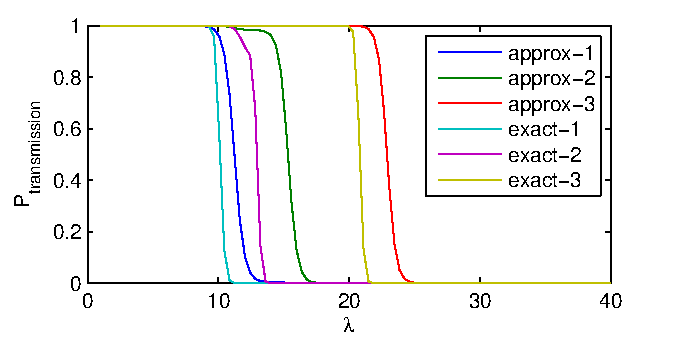
\includegraphics[width=\columnwidth]{results/plotPtransmission_exact_vs_approx.pdf}
  \caption{Comparing the approximate $\Ptrans$ with exact version. The drop in approximate version of $\Ptrans$ is delayed because we assume drop at the center of the car rather than camera facing face of the car.}
  \label{fig:compare:exact:approx:ptrans}
\end{figure}

Thus, we have modeled the transmission probability to effectively capture the effect of occlusion due to all traffic participants in a scene that lie along a particular ray. We reiterate that our reflection and transmission probabilities are continuous functions, which allows us to define continuous energy functions for association and 3D object localization, as described in the next section.

%\paragraph{Probabilistic occlusion levels}
%With the above modeling and using \eqref{eq:imgform}, 



%% We model the probability of a point $\mathbf{x}_j$ on a object $i$ getting successfully
%% observed in a camera image at point $\trackpj{t}$ is dependent up two factors,
%% (1) reflection and (2) transmission through intermediate space. The reflection
%% part ensures that there is an object to reflect a point at a certain region in
%% the 3D space while transmission part models occlusion.
%% \begin{align}
%%   P^{(ij)}_{\text{observation}} = P^{(ij)}_{\text{reflection}}P^{(j)}_{\text{transmission}}
%% \end{align}

%% %%%%%%%%%%%%%%%%%%%%%%%%%%%%%%%%%%%%%%%%%%%%%%%%%%%%
%% \subsection{Reflection probability}
%% For Lambertian reflection we replace the surface normal with the
%% gradient of occupancy.
%% %
%% \begin{align}
%%   \Prefl = (\max \{0, \nabla \occf^\top
%%   \hat{\mathbf{r}_j}\})^2
%% \end{align}
%% %
%% where $\ray =
%% \frac{K^{-1}\trackpj{t}}{\|K^{-1}\trackpj{t}\|}$ is unit vector in the
%% direction of ray. The gradient in the direction opposite to ray yields -ve
%% probability which needs to be clipped off. Squaring the function keep it
%% smooth near zero.

%% %%%%%%%%%%%%%%%%%%%%%%%%%%%%%%%%%%%%%%%%%%%%%%%%%%%%
%% \subsection{Transmission probability}
%% A model for transmission of light through a material of thickness $x$,
%% density $\rho$ and opacity $k_o$ is given by Beer-Lambert law 
%% %
%% \begin{align}
%%   I(x) = I_0e^{-k_o\rho x}
%% \end{align}
%% %

%% Since both opacity and density are represented by the occupancy function
%% $\occftot = \sum_i \occf$, and also the domain of our $\occftot$ is $[0, 1]$ instead of $[0,
%% \infty]$ as in case of $k_o$; we replace $e^{-k_o\rho}$ by the transparency
%% function $1 - \occftot$. So the transmission probability over a small distance
%% $d\lambda$ is given by
%% %
%% \begin{align}
%%   P_{\text{transmission}}(\lambda + d\lambda) =
%%   P_{\text{transmission}}(\lambda) (1-\occftot)^{d\lambda}
%% \end{align}
%% %

%% For a given 3D point $\mathbf{x}_j = \lambda \ray$, the probability that the
%% point $\trackpj{t}$ is reflected from a distance $\lambda$ is given by

%% \begin{align}
%%   %P^{(j)}_{\text{observation}}(\lambda) &= P_{\text{reflection}}
%%   \Ptrans &=
%%   \prod_{0}^{\lambda} (1 - \occft{\lambda \ray})^{d\lambda} %\\
%%   %= \max \{ 0, (\nabla f_{occ}&(\lambda \ray)^\top \ray) \}
%%   %\prod_{0}^{\lambda} (1 - f_{occ}(\lambda \ray))^{d\lambda}
%%   \label{eq:ptrans-integral}
%% \end{align}
%% where $\prod_{0}^{\lambda}$ represents the \emph{product integral} from $0$ to
%% $\lambda$. 

%% In practice, the integral for transmission probability
%% \eqref{eq:ptrans-integral} is difficult to compute even numerically. So we
%% choose a product of sigmoid function that approximates the behaviour of
%% transmission probability,
%% %
%% \begin{align}
%% \label{eq:evalCumulativePtrans}
%%   \Ptrans &= \prod_i L_u(\trackp{t}; \muiu,\Sigmaiu)L_{\lambda}(\lambda; \mu^i_d)
%% \end{align}
%% %
%% where $L_u(.)$ is sigmoid in image domain with $\mu^i_u$ and $\Sigma^i_u$
%% representing the elliptical projection of $i^{th}$ TP.
%% $L_{\lambda}(.)$ is sigmoid in the depth domain with $\mu^i_d$ as the mean
%% depth of the $i^{th}$ TP.
%% %
%% \begin{align}
%%   L_u(\mathbf{u}; \muiu,\Sigmaiu) &= \frac{1}{
%%     1 + e^{-k_u(1 - (\mathbf{u} - \muiu)^\top\Sigmaiu(\mathbf{u} -
%%     \muiu))}
%%   }
%%   \\
%%   L_{\lambda}(\lambda; \mu^i_d) &= \frac{1}{
%%     1 + e^{-k_d(\lambda - \mu^i_d)}
%% }
%% \end{align}
%% %

%% \begin{comment}%% Comment
%%   A product integral is a simple integral in log domain
%%   \begin{align}
%%     \prod_{0}^{\lambda} (1 - f_{occ}(\lambda \ray))^{d\lambda} =
%%     e^{\int_{1}^{\lambda} \ln{(1 - f_{occ}(\lambda \ray))}{d\lambda}}
%%   \end{align}
%% \end{comment}%% Comment

% \paragraph{Notation}
% We summarize the notation used in the report for quick reference.
% \\
% 
% 
%   \begin{tabular}{|l|l|}
%     \hline
%     Symbol & Meaning \\
%     \hline
%     $\pos{i}{t}$ & Position of $i$th car at time $t$\\
%     $\ori{i}{t}$ & Orientation of $i$th car at time $t$\\
%      $\dimsn{i}$ & 3D bounding box of the car (dimensions)\\
%     $\state{i}{t}$ & State of car $=\{\pos{i}{t}, \ori{i}{t}, \dimsn{i}\}$\\
%     $\egop$ & Position of camera at time $t$\\
%     $\egoo$ & Orientation of camera at time $t$\\
%     $\relp{i}{t}$ & Relative car pose w.r.t. camera \\
%     $\tracklets$ & 3D points tracked on car $i$ in its own frame\\
%     $\trackp{t}$ & Projection of $\tracklets$ in camera\\
%     $\projectionOf{.}$ & Projection function for pose $\relp{i}{t}$\\
%     $\bb{i}$ & 2D bounding box of the car in image\\
%     \hline
%   \end{tabular}

\section{Unified Occlusion Models}
%\section{Occlusion-Aware Association and Localization}

In this section, we highlight the versatility of our occlusion modeling by demonstrating its unified application to two different problems: associating point tracks with objects and 3D object localization using object and point tracks.

\subsection{Object-Point Association}
Based on our continuous occlusion model in Section~\ref{sec:setup}, the association probability $\assocP$ of the $j$\textsuperscript{th} point track with $i$\textsuperscript{th} object at depth $\lambda$ can be defined as
\begin{align}
  \assocP = \Prefl\Ptrans,
\end{align}
where $\Prefl$ and $\Ptrans$ are from \eqref{eq:evalPrefl} and \eqref{eq:evalCumulativePtrans} respectively. Note that the fraction $\assocP$ although called association probability does not capture the entire information that we have available for computing association of point tracks to objects. This above fraction is the association probability given the hypothesized parameters of objects in the scene. 

To compute the association probability $\assocP$ between point track $j$ and object $i$, we must use the reprojection error as well. When the association of $i$ and $j$ is correct and the point of reflection is at depth $\lambda$, the reprojection error must be zero \eqref{eq:reprojerror}, otherwise the error becomes a measure of distance from the true solution. The error term can be converted to probability domain by considering the error term as negative log of probability
\begin{align}
  P^{(ij)}_{\text{assoc by reproj}}(\lambda) = \frac{1}{Z}\exp(-\Ereproj(\lambda))
\end{align}

Using both of the above evidence terms we can write the probability of association $P^{(ij)}_{\text{assoc}}$ as follows
\begin{align}
  P^{(ij)}_{\text{assoc}} = \frac{1}{Z'}\int_0^{\infty} \assocP \exp(-\Ereproj(\lambda))d\lambda
  \label{eq:prob-assoc}
\end{align}
Once we have the probability of association $P^{(ij)}_{\text{assoc}}$ we can compute the best possible assignment of object for each point track. The points having very small association probability are assigned to the background,
\begin{align}
  i^*_{j} = \arg \min_{i} \int_0^\infty \assocP \Ereproj(\lambda) d\lambda
\end{align}


In contrast to the principled approach above, a heuristic baseline may simply assign a point to the detection bounding box enclosing it (and background if outside all bounding boxes). For regions where bounding boxes overlap, it may assign point tracks to the object that has smaller mean depth among the competing bounding boxes. As we will demonstrate in experiments, such heuristics are sub-optimal compared to using \eqref{eq:prob-assoc} inspired by our occlusion model.

%For the baseline method, the associations between point tracks and TPs are achieved by using detection bounding boxes, where point tracks within each bounding box are simply assigned to it. For the regions where the bounding boxes overlap, we assign the point tracks to the TP that has smaller mean depth than the competing bounding boxes.



\subsection{3D Object Localization}
To show the effectiveness of our method we apply it to the localization
problem. We estimate the position, orientation and dimensions of the car with
our framework and compute the error in birds eye view domain along the ground
plane. We report error in three metrics translation error (t) in meters per
car, yaw error (yaw) in radians per car and dimension error is again meters per
car. The results are shown in Table~\ref{tab:localizationExperiment}.

We build the graphical model as shown in Fig~\ref{fig:graphmodel} that 
allows us to factorize the intractable probability distribution into following form
%
\begin{multline}
  -\log{P(\{\state{i}{t}\} | \mathbb{E})} = 
  -Z' 
  \\
  + \sum_{t=s_i}^{e_i}
  \left(
  \sum_{i,j:i\ne j}   
  \WEnergyCol 
   + \WpEnergy{bbox}
   + \WpEnergy{track}
\right)
  \\
  + \left(
  \sum_{i=1}^N 
  \WEnergy{lane}
  + \WEnergy{dyn}
  + \WEnergy{size}
\right)
  \enspace.
\end{multline}
%
Next, we explain the important energies used in our graphical model.

\subsubsection{Continuous point tracks energy with occlusion}
\label{sec:totalContPtTracksEnergy}
We model continuous point tracks energy with explicit occlusion reasoning as
the expected reprojection error over the association probability,

\begin{multline}
  \Energy{track}(\{ \relp{i}{t} \}_i, \{ \relp{i}{t-1} \}_i, \{\dimsn{i}\}_i ) = 
  \\
    \sum_{i=1}^{N} 
    %\sum_{t = s_i}^{e_i}
    \sum_{j = 1}^{M}
    \int_1^\infty \assocP\Ereproj(\lambda) d\lambda
\end{multline}
where $\assocP$ is the association probability of
$j$\textsuperscript{th} point with $i$\textsuperscript{th} TP at depth $\lambda$, $\{ \relp{i}{t} \}_i$ are the poses of all occluding objects at time $t$, $ \{ \dimsn{i} \}_i$ are the dimensions of all objects that occlude $i$
and $\Ereproj(\lambda)$ is the reprojection error given by
%
\begin{align}
  \assocP &= \Prefl\Ptrans\\
  \Ereproj(\lambda) &= \left\|\trackpj{t} - \projectionOf{\invProjectionOftm{\trackpj{t-1}, \lambda}}\right\|^2 .
  \label{eq:reprojerror}
\end{align}

The  $\projectionOf{.}$ and $\invProjectionOftm{.}$ denote the projection and
inverse projection functions that project 3D point to camera image and vice
versa. Note that inverse projection $\invProjectionOf{.}$ depend on both the
point $\trackp{t}$ and the unknown depth $\lambda$. Also note that the inverse projection is dependent on TP pose at time $t-1$ while the projection depends on pose at time $t$ which can be different.

\subsubsection{Continuous bounding box energy with occlusion}

Object detection is usually followed by non-maximal suppression that results in
discarding similar bounding boxes. When we are jointly optimizing detections
with other cues, it is not usually desirable to go with a single bounding box.
Hence, we keep all the bounding box detections by approximating them with
multi-modal sum of Gaussian like logistic functions. We fit the parametric function of the form 
%
\begin{multline}
  S(\bb{i}) = \\
  \sum_k A_k \exp(-(\bb{i}-\mu^{(d)}_k)^\top \Sigma^{(d)-1}_k
  (\bb{i}-\mu^{(d)}_k))
\end{multline}
%
to detection scores, by non-linear error minimization with initialization from
non-maximal suppressed outputs. Here $\mu^{(d)}_j$ is one of the $k$ modes as a
4D vector representing a single bounding box as $[\minx, \miny, \maxx,
\maxy]^\top$. The optimization is constrained with symmetry and positive
definiteness of $\Sigma^{(d)-1}_k$, $\maxx \ge \minx$ and $\maxy \ge \miny$.

\paragraph{Detection scores with occlusion reasoning} 
\def\u{\mathbf{u}}
With our model of $\Ptrans$ described in Section \ref{sec:ptransmission}, we can
compute the probability of a point $\u$ on image be occluded assuming
the point is on traffic participant (TP) $i$ with mean depth $\mu^{(i)}_d$ as
\begin{align}
  O_{i}(\u, \mu^{(i)}_d) = 1 - \Ptransmission(\mu^{(i)}_d\u) \enspace .
\end{align}

If we know a portion of our proposed detection bounding box is known to be
occluded, then we would like to decrease the confidence in the detection score
about the localization of that end of the object. Assuming that the occlusion
is often on the boundary of detection bounding boxes, we want to decrease our
confidence on the mean detection boundaries around the occluded boundaries.
To re-model our detection scores scaled by continuous occlusion we sample
$O_{i}(\mathbf{u}, \mu^{(i)}_d)$ at the hypothesized detection boundaries from
GMM $S(.)$ and we augment the detection boundary covariance matrix by
$\mathcal{P}_{j} = \rho_{j}\rho_{j}^\top$ where $\rho_{j} = O_{j}(\mathbf{u},
\mu^{(i)}_d)$. The new covariance matrix in detection score is given by 
  $\Sigma'^{(d)}_j = \mathcal{P}_{j} + \Sigma^{(d)}_j$.
The detection scores GMM with occlusion is given by replacing the covariance
matrix
%
\begin{multline}
  S'(\bb{i}) =
  \\
  \sum_j A_j \exp(-(\bb{i}-\mu^{(d)}_j)^\top \Sigma'^{(d)-1}_j
  (\bb{i}-\mu^{(d)}_j))
\end{multline}

The energy of detection scores is simply take to be the inverse of the detection score.
\begin{align}
  \Energy{detect}(\{ \relp{i}{t} \}_i, \{ \relp{i}{t-1} \}_i, \{\dimsn{i}\}_i ) = \frac{1}{S'(\bb{i})}
\end{align}

For object detections we use object detector by \cite{Felzenszwalb_etal_2010}
which is detector by parts model and we use eight parts to train the car model 
on half of the KITTI dataset \cite{geiger2013vision}. The trained modeled is 
used to get detections for the other half of the dataset and vice versa. 

\subsubsection{Other energies}
Other energies we use are described in detail in the supplementary material. We briefly describe them here:
\begin{description}
  \item[Lane energy ($\Energy{lane}$)] This energy term constrains the
    orientation of traffic participants to be parallel to the nearest detected
    lane. The lanes are either detected visually or obtained from GPS and Map 
    information.
  \item[Transition probability ($\Energy{dyn}$)] We use these energies to
    constrain the motion of cars to be smooth in linear motion and rotation
    motion. We also constrain cars to move in the direction of heading.
  \item[Size prior ($\EnergySize$)] We use size prior of cars by using the mean
    of cars over the KITTI dataset.
\end{description}

\subsection{Metropolis Hastings Inference}
We use Metropolis Hastings' methods for graphical model inference. Since we are
optimizing over continuous random variables, we use Gaussian distribution as
the proposal distribution.

\begin{figure}
  \centering
  \newcommand{\imagewidth}{\columnwidth}
  ../../CVPR/Source/scenelayoutoverlayCity0961.tex
  \caption{A sample road scene with the unknowns of each car modeled as random variables. 
  The relating energies are shown in Figure~\ref{fig:graphmodel}}
\end{figure}
\begin{figure}
    \usetikzlibrary{trees,shadows}
\begin{tikzpicture}[grow cyclic, line width=1.2pt,
    variablenode/.style={circle,circular drop shadow,draw=red,fill=white,thick,minimum width=0.5cm},
   bboxfactor/.style={rectangle,drop shadow,draw=green,fill=green,thick,minimum width=0.2cm},
    collfactor/.style={rectangle,drop shadow,draw=blue,fill=blue,thick,minimum width=0.2cm},
    trackfactor/.style={rectangle,drop shadow,draw=red,fill=red,thick,minimum width=0.2cm},
  obs/.style={fill=gray!30,draw=black},
  prevf/.style={draw=green!20,text=gray},
  prevobsv/.style={draw=gray!10,fill=gray!1,text=gray},
  prevv/.style={draw=red!20,text=gray}
]
  \path[use as bounding box,clip] (-2.5, -5.5) rectangle (5.5,0.5);
  \draw (-2.5,-2.65) rectangle +(0.5,0.3);
  \draw (-2.0,-2.35) -- ++(0.15, 0.15) -- ++(0, -0.6) -- (-2.0, -2.65);
\path
     (0, 0)  node [variablenode] (x6) {6}
++(0, -1.5) node [variablenode] (x2) {2}
++(2.5, 0)  node [variablenode] (x5) {5}
+ (0, 1.5)  node [variablenode,obs] (u) {}
+(.2,1.0)  node {$u$}
+ (.5, -2)   node [variablenode] (x3) {3}
+ (2.3, -3.5)   node [variablenode] (x4) {4}
+(2.5, 0)  node [variablenode] (x1) {1}
;

% Factors between nodes 6 and 2
\draw (x6) edge [bend right=35] node [bboxfactor] (f26) {} (x2);
\path (f26) +(-0.75,0) node [variablenode,obs] (d6) {} 
                        +(-.7,-.6)  node {$d^6$};
\draw (f26) edge (d6);
\draw (x6) edge [bend left=35] node [trackfactor] (ft26) {} (x2);
\draw (ft26) edge [bend left=10] (u);
\draw (x6) edge node [collfactor] {} (x2);

% Factors for node 2
\path (x2) +(0,-1.25) node [variablenode,obs] (d2) {} 
                        +(-.6,-1.3)  node {$d^2$};
\draw (x2) edge node [bboxfactor] {} (d2);

% Factors between nodes 2 and 5
\draw (x2) edge [bend right] node [bboxfactor] (f25) {} (x5);
\draw (x2) edge [bend left] node [trackfactor] (ft25) {} (x5);
\draw (x2) edge [] node [collfactor] {} (x5);
\draw (ft25) edge (u);
\path (x5) ++(-1.25,-1.25) node [variablenode,obs] (d5) {} 
                        +(.6,0)  node {$d^5$};
\draw (f25) edge (d5);

% Factors between nodes 5 and 1
\draw (x5) edge [bend right] node [bboxfactor] (f51) {} (x1);
\draw (x5) edge [bend left] node [trackfactor] (ft51) {} (x1);
\draw (x5) edge [] node [collfactor] {} (x1);
\draw (ft51) edge [bend right] (u);
\path (x1) ++(-1.25,-1.25) node [variablenode,obs] (d1) {} 
                        +(-.5,0.2)  node {$d^1$};
\draw (f51) edge (d1);

% Factors for node 3
\path (x3) ++(0,-1.25) node [variablenode,obs] (d3) {} 
                        +(.6,0)  node {$d^3$};
\draw (x3) edge node [bboxfactor] {} (d3);

% Factors for node 4
\path (x4) ++(0,1.25) node [variablenode,obs] (d4) {} 
                        +(.6,0)  node {$d^4$};
\draw (x4) edge node [bboxfactor] {} (d4);

% Legend
\path (-1.75,-4.0) node (l1s) {} (-0, -4.0) node [anchor=west] (l1e) {$\Energy{bbox}$};
\draw (l1s) edge node [bboxfactor] {} (l1e);
\path (-1.75,-4.5) node (l2s) {} (0, -4.5) node [anchor=west] (l2e) {$\EnergyCol$};
\draw (l2s) edge node [collfactor] {} (l2e);
\path (-1.75,-5.0) node (l3s) {} (0, -5.0) node [anchor=west] (l3e) {$\Energy{point}$};
\draw (l3s) edge node [trackfactor] {} (l3e);

\end{tikzpicture}

    \caption{Graphical model for a single frame with state of car represented
    as single node.  The six numbered nodes represent the unknown state variables of each car. The shaded nodes in the graphical model are observed variables. }
  \label{fig:graphmodel}
\end{figure}

\section{Experiments}
\label{sec:experiments}

In this section, we benchmark our continuous occlusion model for point-to-object association against the baseline method using detection bounding boxes and state-of-the-art methods for motion segmentation \cite{Rao_etal_2010,Brox_Malik_2010}. We then show how the proposed model may be applied for 3D object localization in road scenes. For our experiments, we use 35 sequences of the KITTI raw dataset~\cite{Geiger_etal_2012}, which are recorded under a variety of driving conditions and include 10,088 frames and 634 object tracks in total. 
%It also provides ground truth data for different tasks such as segmentation, detection, tracking and 3D localization.

%\paragraph{Dataset} We use KITTI dataset for our experiments.  \cite{geiger2013vision}. KITTI dataset is a labeled video sequence of road scenes under variety of driving conditions including highways and residential areas in Karlsruhe, Germany. It provides manually labelled ground truth data for localization of cars and also uses velodyne data provide metrically accurate estimates of cars location.


%%%%%%%%%%%%%%%%%%%%%%%%%%%%%%%%%%%%%%%%%%%%%%%%%%%%



\subsection{Association Experiments}
%\vspace{-0.2cm}
\paragraph{Setup}
We first perform the association experiment that compares the accuracy of point-to-object association using our proposed model against a heuristic baseline and state-of-the-art motion segmentation methods. The detection bounding box baseline method (BBox) is as described at the end of Section \ref{sec:association}. For motion segmentation, we use robust algebraic segmentation with hybrid perspective constraints (RAS)~\cite{Rao_etal_2010} and spectral clustering with point track spatial affinities (BM)~\cite{Brox_Malik_2010}.


\begin{figure*}[!!t]
\centering
%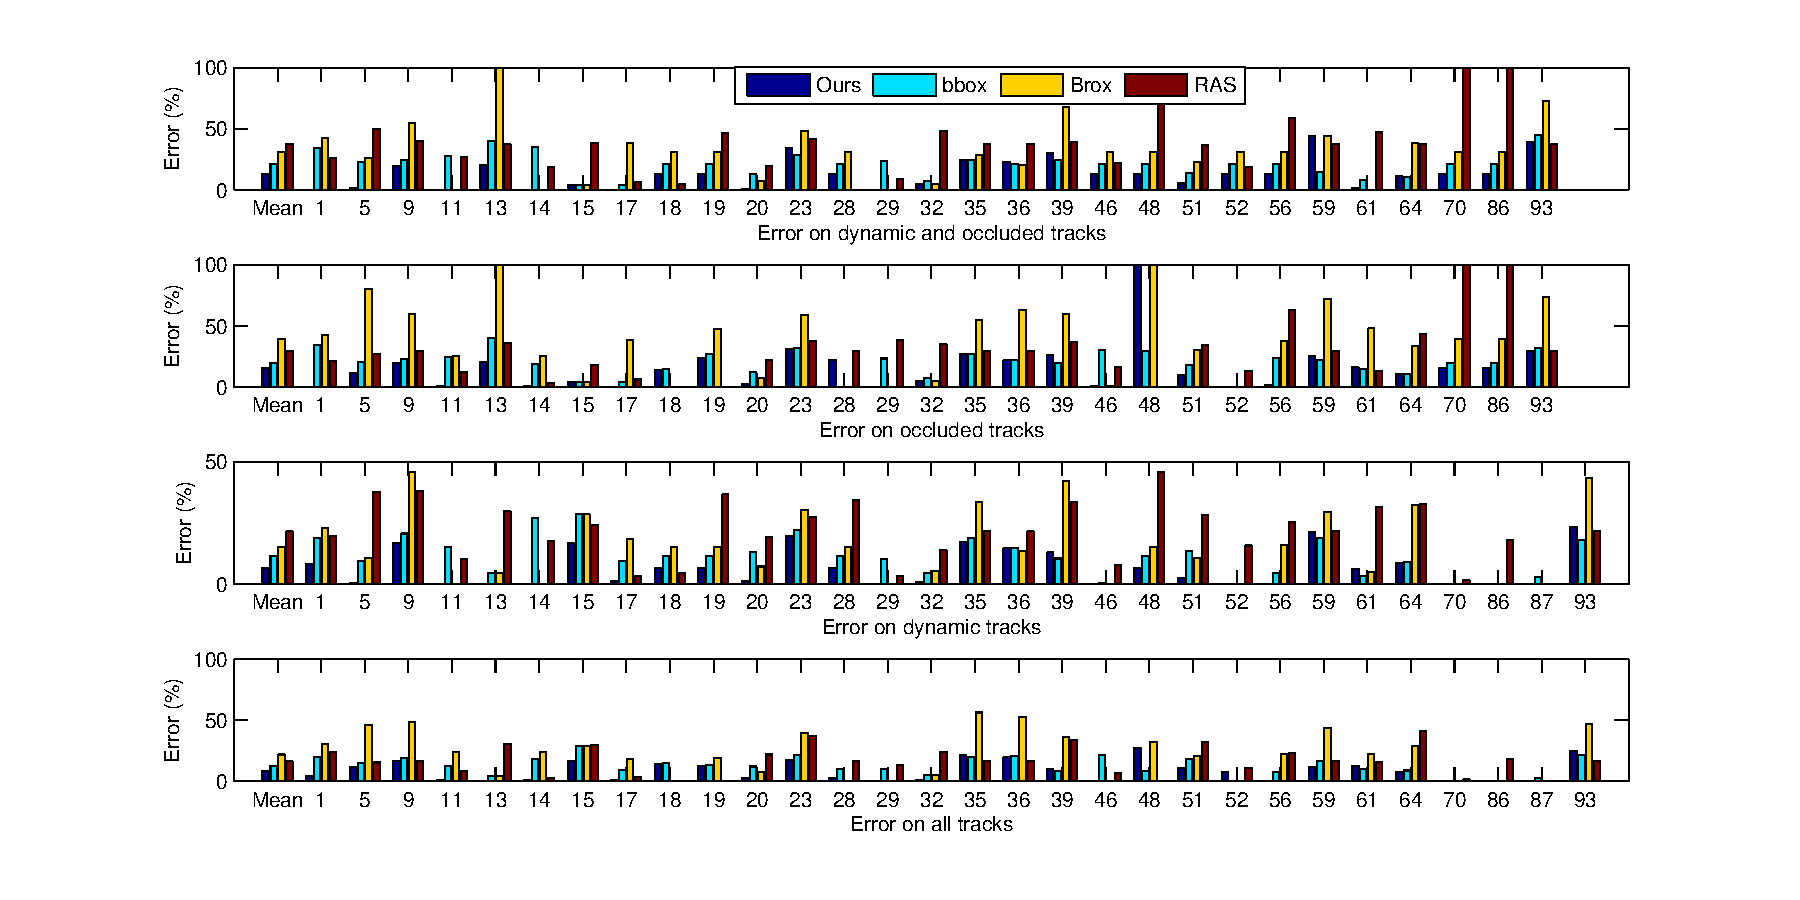
\includegraphics[trim=1.0in 0.4in 1.0in 0.2in, clip, width=\textwidth]{results/plotErrorBarEvalAssocCoeffAllSequence.pdf}
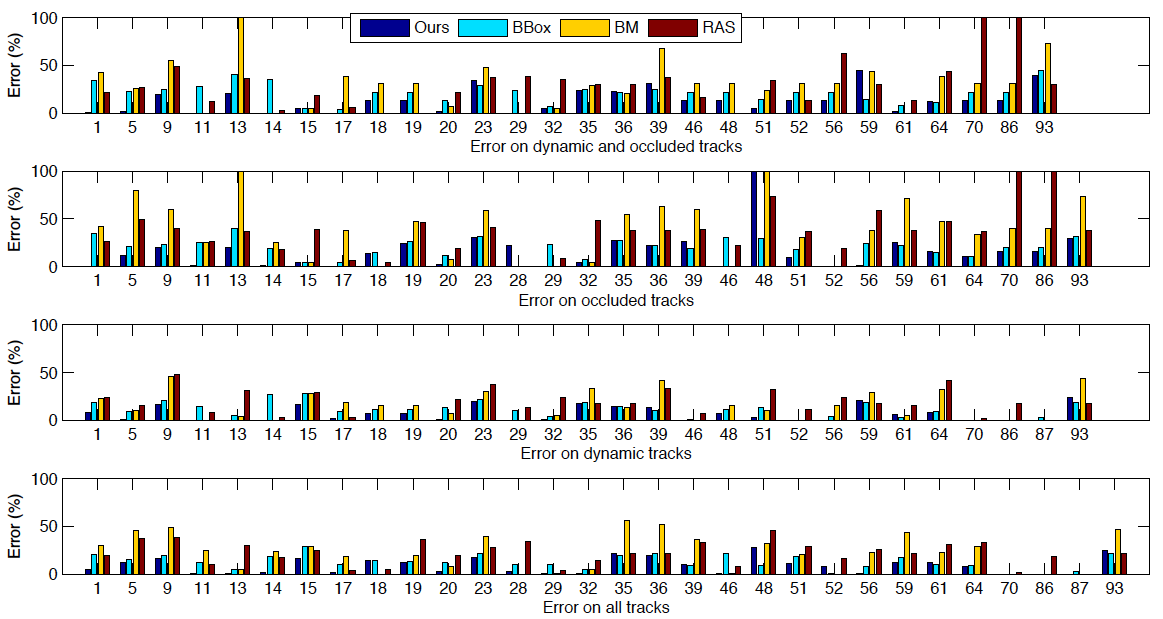
\includegraphics[width=0.95\textwidth]{graphics/figure5.png}
  \vspace{-0.3cm}
  \caption{\small Association errors on different sets of input point tracks. Numbers on x-axis represent sequence numbers in the KITTI raw dataset. Errors are in terms of average fractions of foreground points incorrectly associated to objects per sequence.}
  \vspace{-0.3cm}
  \label{fig:assoc-occ-results}
\end{figure*}

\begin{table}
\begin{tabular}{lrrrr}
  \toprule
  Point tracks & Ours & BBox & BM & RAS\\
  \midrule
  Dynamic \& occluded         & \textbf{13.2} & 21.3 & 30.9 & 30.1 \\
  Occluded		              & \textbf{15.7} & 19.8 & 39.5 & 37.8 \\
  Dynamic		              & \textbf{6.6} & 11.4 & 15.3 & 17.7 \\
  All		                  & \textbf{8.6} & 12.6 & 21.9 & 21.5 \\
  \bottomrule
\end{tabular}
\caption{\small Mean association errors on different sets of input point tracks over all sequences. Errors are in terms of average fractions of foreground points incorrectly associated to objects per sequence.}
\label{tab:meanAssoc}
\end{table}


\newlength{\tblimgwidth}
\setlength{\tblimgwidth}{0.090\textwidth}
\begin{figure*}[!!t]
  \centering
  \begin{tabular}{cc@{}c@{\hspace{0.1cm}}c@{}c@{}}
    & Associations & Errors & Associations & Errors\\
    \rotatebox{90}{\hspace{1em} BBox}%
    & 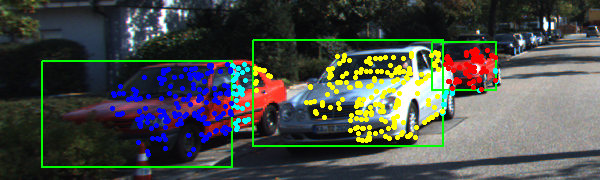
\includegraphics[height=\tblimgwidth]{results/0009_0000000060_point_assign_bbox2D_model-small.png}%
    & 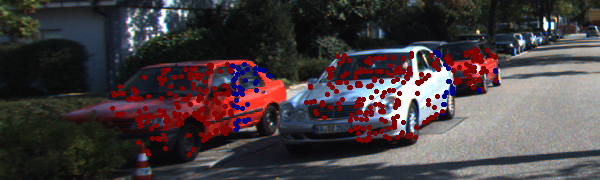
\includegraphics[height=\tblimgwidth]{results/0009_0000000060_point_assign_bbox2D_model_correct_incorrect-small.png}%
    & 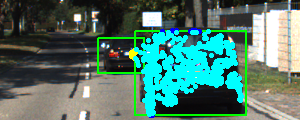
\includegraphics[height=\tblimgwidth]{results/0013_0000000060_point_assign_bbox2D_model-small.png}%
    & 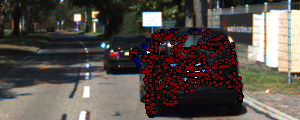
\includegraphics[height=\tblimgwidth]{results/0013_0000000060_point_assign_bbox2D_model_correct_incorrect-small.png}\\
    \rotatebox{90}{\hspace{1em} BM}%
    & 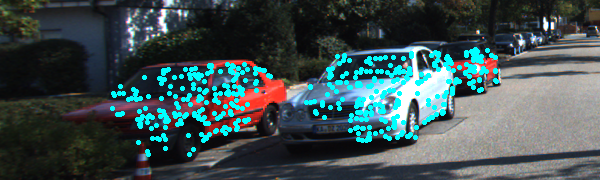
\includegraphics[height=\tblimgwidth]{results/0009_0000000060_point_assign_BroxAndMalik2010-small.png}%
    & 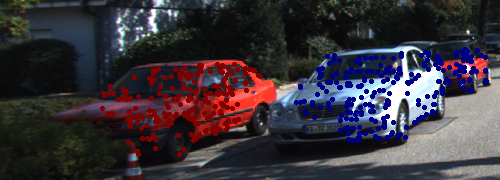
\includegraphics[height=\tblimgwidth]{results/0009_0000000060_point_assign_BroxAndMalik2010_correct_incorrect-small.png}%
    & 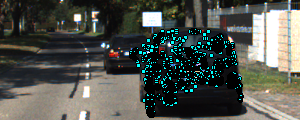
\includegraphics[height=\tblimgwidth]{results/0013_0000000060_point_assign_BroxAndMalik2010-small.png}%
    & 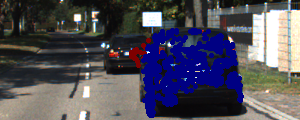
\includegraphics[height=\tblimgwidth]{results/0013_0000000060_point_assign_BroxAndMalik2010_correct_incorrect-small.png}\\
    \rotatebox{90}{\hspace{1em} RAS}%
    & 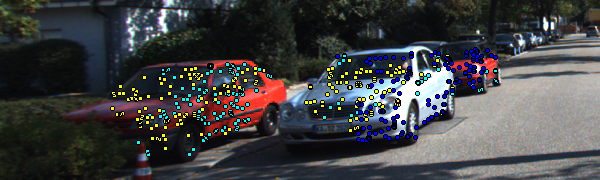
\includegraphics[height=\tblimgwidth]{results/0009_0000000060_point_assign_RAS-small.png}%
    & 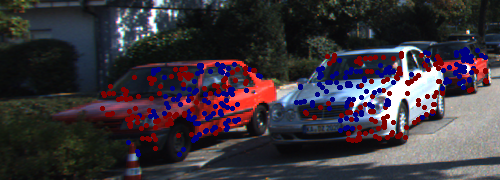
\includegraphics[height=\tblimgwidth]{results/0009_0000000060_point_assign_RAS_correct_incorrect-small.png}%
    & 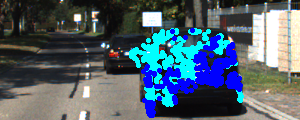
\includegraphics[height=\tblimgwidth]{results/0013_0000000060_point_assign_RAS-small.png}%
    & 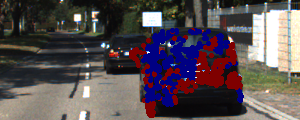
\includegraphics[height=\tblimgwidth]{results/0013_0000000060_point_assign_RAS_correct_incorrect-small.png}\\
    \rotatebox{90}{\hspace{1em} Ours}%
    & 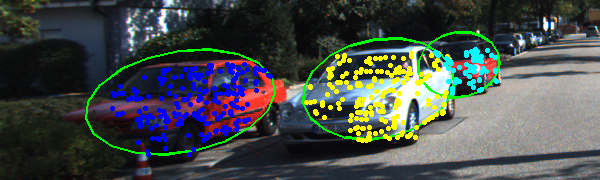
\includegraphics[height=\tblimgwidth]{results/0009_0000000060_point_assign_contPtTracks-small.png}%
    & 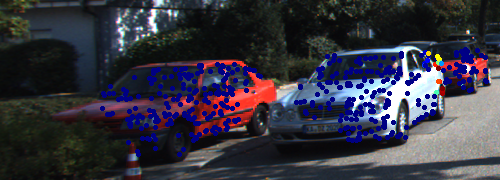
\includegraphics[height=\tblimgwidth]{results/0009_0000000060_point_assign_contPtTracks_correct_incorrect-small.png}%
    & 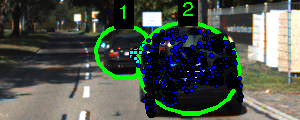
\includegraphics[height=\tblimgwidth]{results/0013_0000000060_point_assign_contPtTracks-small.png}%
    & 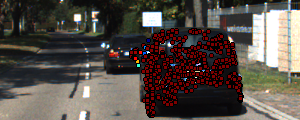
\includegraphics[height=\tblimgwidth]{results/0013_0000000060_point_assign_contPtTracks_correct_incorrect-small.png}
  \end{tabular}
  \vspace{-0.3cm}
  \caption{\small Qualitative results of the association experiment. The ``Associations" columns
  show the point track assignments to appropriate objects. Each color represents
a different object to which point tracks can be associated to. The ``Errors" columns show the
probabilistic errors in association: low error points are in blue while high error points are in red.
Note that our method changes smoothly at the object boundaries with
intermediate probabilities, while the baseline method has merely 0 and 1 errors.}
\label{fig:qualitative}
\vspace{-0.3cm}
\end{figure*}


%To verify the correctness of our association probability $\assocP$ we perform association error experiment that compare the accuracy of point track association with TPs with that of bounding box baseline method.

For each sequence, the methods of \cite{Felzenszwalb_etal_2010} and \cite{Choi_Savarese_2010} are used for computing detection bounding boxes and object tracklets, respectively. We then apply \cite{Zach2007} to extract point tracks. Note that our method can handle occlusions in both static and dynamic scenes, but motion segmentation focuses on dynamic scenes. For a complete evaluation, we organize the point tracks into four sets: all point tracks, occluded point tracks, dynamic point tracks and dynamic as well as occluded point tracks. The parameters (position, orientation, and dimensions) of all objects (cars) estimated by the method of \cite{Song_Chandraker_2014} are provided to our method (for computing association probability) and the baseline BBox method (for depth ordering). The number of objects is known a priori in our model (from object tracking~\cite{Choi_Savarese_2010}) and is also provided to other methods such as BBox and RAS.

\vspace{-0.4cm}
\paragraph{Results}
Figure~\ref{fig:assoc-occ-results} shows the association errors -- the percentages of point tracks incorrectly assigned to objects -- for all methods on the four sets of input point tracks, for each sequence. The mean results over all sequences are summarized in Table~\ref{tab:meanAssoc}. From Figure~\ref{fig:assoc-occ-results}, our method is usually the most accurate among all methods, leading to the best mean error on all sets of input point tracks in Table~\ref{tab:meanAssoc}, which is followed by the bounding box baseline method. This clearly shows the advantage of our continuous occlusion model over the simple baseline method for resolving occlusions. RAS and BM often have the highest errors in Figure~\ref{fig:assoc-occ-results}, thus, the highest mean errors on all sets of input point tracks in Table~\ref{tab:meanAssoc}. 

More importantly, both RAS and BM rely on motions of objects for clustering point tracks, therefore they cannot work well with static point tracks (for example, point tracks that belong to parked cars). This fact can be observed in Table~\ref{tab:meanAssoc}, where there are large differences in the mean errors of both methods on data containing static point tracks (rows 2 and 4) and data consisting of dynamic point tracks only (rows 1 and 3). In contrast, our method and the baseline method are relatively independent of object motions, resulting in smaller performance gaps. Further, our method also outperforms motion segmentation on dynamic objects (row 3), which shows the effect of detection bounding boxes and by a more significant margin when occlusions are present (row 1), which shows the effect of our occlusion modeling.

Qualitative comparisons of point track associations from various methods are shown in Figure \ref{fig:qualitative}. We note the low errors using our occlusion model and the smooth transition of assignment across object boundaries.



%  seqName   seqNum    Energy_description                                                    windows         t      yaw             dim        
%    City      1       contPtTracksNoOcc_ctBBoxNoOcc_size_posTmcmc_inference      9/18  5.811142 0.696358        1.961227        
%    City      1       contPtTracksNoOcc_contBBoxOcc_size_posTmcmc_inference      8/18  4.501543 0.786599        2.375481        
%    City      1       contPtTracks_ctBBoxNoOcc_size_posTmcmc_inference           8/18  3.932855 0.766397        2.222919        
%    City      1       contPtTracks_contBBoxOcc_size_posTmcmc_inference           8/18  4.928155 0.806356        2.287911        
% OccCity      1       contPtTracksNoOcc_ctBBoxNoOcc_size_posTmcmc_inference      9/18  3.953464 0.442196        1.720844        
% OccCity      1       contPtTracksNoOcc_contBBoxOcc_size_posTmcmc_inference      8/18  4.815849 0.463034        2.159956        
% OccCity      1       contPtTracks_ctBBoxNoOcc_size_posTmcmc_inference           8/18  4.058560 0.995495        1.593641        
% OccCity      1       contPtTracks_contBBoxOcc_size_posTmcmc_inference           8/18  3.241853 0.631901        2.167446        
% \begin{table}
%   \centering
%   \begin{tabular}{lrrr}
%     \toprule
%     Energy & t & yaw & dim \\
%     \midrule
%     $\EnergyTrackNoOcc + \EnergyBBoxNoOcc +\EnergySize+\EnergyDyn$
%     5.81 & 0.69 & 1.96 \\
%     $\EnergyTrackNoOcc + \EnergyBBox +\EnergySize+\EnergyDyn$
%     4.50 & 0.78 & 2.37 \\
%     $\EnergyTrack + \EnergyBBoxNoOcc +\EnergySize+\EnergyDyn$
%     3.93 & 0.76 & 2.22 \\
%     $\EnergyTrack + \EnergyBBox +\EnergySize+\EnergyDyn$
%     4.92 & 0.80 & 2.28 \\
%     \bottomrule
%   \end{tabular}
%   \caption{Localization experiment results with different combination of energies. We report error in three metrics translation error (t) in meters per car, yaw error (yaw) in radians per car and dimension error is again meters per car.}
%   \label{tab:localizationExperimentNoOcc}
% \end{table}

%% \begin{table}
%% \small
%%   \begin{tabular}{lrrr}
%%     \toprule
%%     Energy & t & yaw & dim \\
%%     \midrule
%%     $\EnergyTrackNoOcc + \EnergyBBoxNoOcc +\EnergySize+\EnergyDyn$ 
%%     & 3.95 & 0.44  & 1.72\\        
%%     $\EnergyTrackNoOcc + \EnergyBBox +\EnergySize+\EnergyDyn$        
%%     & 4.81 & 0.46  & 2.16\\        
%%     $\EnergyTrack + \EnergyBBoxNoOcc +\EnergySize+\EnergyDyn$      
%%     & 4.05 & 0.99  & 1.59\\        
%%     $\EnergyTrack + \EnergyBBox +\EnergySize+\EnergyDyn$             
%%     & 3.24 & 0.63  & 2.16\\
%%     \bottomrule
%%   \end{tabular}
%%   \caption{\small Localization experiment results with different combination of energies. We report error in three metrics translation error (t) in meters per car, yaw error (yaw) in radians per car and dimension error is again meters per car. The results provided here are only on occluded tracks.}
%%   \label{tab:localizationExperiment}
%% \end{table}


\begin{table}
  \begin{tabular}{lrr}
    \toprule
    Method & t & dim \\
    \midrule
    Point cloud fitting
    & 6.87 & 4.02\\
    Initialization
    & 5.61 & 3.23\\
    $\EnergyTrackNoOcc + \EnergyBBoxNoOcc +\EnergySize+\EnergyDyn$ 
    & 3.95  & 1.72\\        
    $\EnergyTrackNoOcc + \EnergyBBox +\EnergySize+\EnergyDyn$        
    & 4.81  & 2.16\\        
    $\EnergyTrack + \EnergyBBoxNoOcc +\EnergySize+\EnergyDyn$      
    & 4.05  & {\bf 1.59}\\        
    $\EnergyTrack + \EnergyBBox +\EnergySize+\EnergyDyn$             
    & {\bf 3.24}  & 2.16\\
    \bottomrule
  \end{tabular}
  \caption{\small Localization experiment results with different combinations of energies. We report translation error (t) and dimension error (dim) in meters per car. Yaw angles for static objects are not optimized by our model. These experiments use the set of occluded tracks to demonstrate the effect of our modeling.}
  \label{tab:localizationExperiment}
\end{table}


\subsection{Localization Experiments}
We report errors in translation and dimension estimates, measured in meters per car, in Table~\ref{tab:localizationExperiment}. Average depth of cars in the dataset is approximately $20$ meters. We compare four combinations of energies against the initialization by~\cite{Song_Chandraker_2014} and a simple baseline which fits a 3D cuboid on the 3D point cloud reconstructed using SFM within detection bounding boxes in consecutive frames (for unobservable dimensions, e.g., only the back of a car is visible, we rely on 3D size priors). The energy $\EnergyTrackNoOcc$ represents the point track energy without accounting for occlusion, that is, we model $\EnergyTrack$ in the absence of $a^{ij} (\lambda)$. Similarly, $\EnergyBBoxNoOcc$ is the bounding box energy without the modification of $\bLambda_k$ that accounts for occlusion.

From Table~\ref{tab:localizationExperiment}, the baseline method has the highest errors, which is likely due to lack of point tracks and incorrect point-to-object associations (using detection bounding boxes). Moreover, minimizing different combinations of energies yields lower errors than the initialization by~\cite{Song_Chandraker_2014}, which shows the advantage of our energy minimization. Finally, we observe that the use of the continuous occlusion model improves the localization accuracy in terms of the translation error, which is the most significant metric affected by all cues. Occlusion modeling for detection increases dimension error since we explicitly allow greater uncertainty in occluded edges of the bounding box. Note that none of our energies optimize yaw angles for static objects, which can be handled in practice through either the detector orientation or external information such as lane geometry.


%We report errors in translation and dimension estimates, measured in meters per car, in Table~\ref{tab:localizationExperiment}. Average depth of cars in the dataset is approximately $20$ meters. We compare four combinations of energies with two baselines. We initialize the unknowns using \cite{Song_Chandraker_2014} whose accuracy is reported as \emph{Initialization} in the table. We develop a simple baseline by fitting cuboids to the point cloud created by triangulation of point tracks in two successive frames. The accuracy of this baseline is reported as \emph{Point cloud fit} in the table. The energy $\EnergyTrackNoOcc$ represents the point tracks energy without accounting for occlusion, that is, we model $\EnergyTrack$ in the absence of $a^{ij} (\lambda)$. Similarly, $\EnergyBBoxNoOcc$ is the energy without the modification of $\Lambda_k$ that accounts for occlusion. We observe that the use of the continuous occlusion model improves the localization accuracy in terms of the translation error, which is the most significant metric affected by all cues. Occlusion modeling for detection increases dimension error since we explicitly allow greater uncertainty in occluded edges of the bounding box. Note that none of our energies optimize yaw angles for static objects, which can be handled in practice through either the detector orientation or external information such as lane geometry.

%of all three metrics: translation, yaw and dimension error.


%We report error in three metrics translation error (t) in meters per car, yaw error (yaw) in radians per car and dimension error is again meters per car. The results are shown in Table~\ref{tab:localizationExperiment}.  We compare four combinations of energies as shown in the table.  The energy $\EnergyTrackNoOcc$ represents the point tracks energy modeled with accounting for occlusion, i.e., we remove the term $\Ptransmission$ and model $\EnergyTrack$ in the absence of $\Ptransmission$. Similarly, $\EnergyBBoxNoOcc$ is the energy without the modification of $\Sigma^{(d)}_j$ that accounts for occlusion.  The results show that use of continuous occlusion model improves the localization accuracy in terms of all three metrics: translation, yaw and dimension error.


\section{Discussion and Future Work}
\label{sec:discussions}

Our experiments shows that our association probability produces more accurate point to object associations when compared to simple bounding box based association. This shows that our occlusion aware 3D representation of objects works. However the localization experiment results do not show significant improvements by using more complicated models. 

% \section{Possible sources of error}
Since the results are averaged over the entire KITTI dataset, there are various possible sources of error, including outliers in point tracks, outliers in detections results. By noting that the dimension error is lower for fewer energies and translation error follows a relatively unpredictable trend, we stress on the requirement of learning of energy weights $\lambda_{\text{col,bbox,track,lane,dyn,size}}$. However, because of slow inference algorithms, which take about a day to run on 300 cores for the entire KITTI dataset, learning become infeasible.

%\section{Possible ways of improving the results}
We have several ideas for speeding up inference and thereby allowing learning
of weights to become feasible. One of them is to approximate the graph into a tree using Chow-Liu's \cite{chow1968approximating} algorithm and then using Belief Propagation which is linear in the number of edges of the tree.


%\section*{Acknowledgements}
%Vikas Dhiman and Jason J. Corso are partially supported by the National Science Foundation through the grant NRI IIS 1522904.





%{\small
%\bibliographystyle{ieee}
%\bibliography{continuousocclusion}
%}
%\end{document}
